\documentclass[10pt,landscape]{scrartcl}
\usepackage{multicol}
\usepackage{calc}
\usepackage{ifthen}
\usepackage[landscape]{geometry}
\usepackage{amsmath,amsthm,amsfonts,amssymb}
\usepackage{color,graphicx,overpic}
\usepackage{hyperref}
\usepackage{graphicx}


% This sets page margins to .5 inch if using letter paper, and to 1cm
% if using A4 paper. (This probably isn't strictly necessary.)
% If using another size paper, use default 1cm margins.
\ifthenelse{\lengthtest { \paperwidth = 11in}}
    { \geometry{top=.5in,left=.5in,right=.5in,bottom=.5in} }
    {\ifthenelse{ \lengthtest{ \paperwidth = 297mm}}
        {\geometry{top=1cm,left=1cm,right=1cm,bottom=1cm} }
        {\geometry{top=1cm,left=1cm,right=1cm,bottom=1cm} }
    }

% Turn off header and footer
\pagestyle{empty}

% Redefine section commands to use less space
\makeatletter
\renewcommand{\section}{\@startsection{section}{1}{0mm}%
                                {-1ex plus -.5ex minus -.2ex}%
                                {0.5ex plus .2ex}%x
                                {\normalfont\large\bfseries}}
\renewcommand{\subsection}{\@startsection{subsection}{2}{0mm}%
                                {-1explus -.5ex minus -.2ex}%
                                {0.5ex plus .2ex}%
                                {\normalfont\normalsize\bfseries}}
\renewcommand{\subsubsection}{\@startsection{subsubsection}{3}{0mm}%
                                {-1ex plus -.5ex minus -.2ex}%
                                {1ex plus .2ex}%
                                {\normalfont\small\bfseries}}
\makeatother

% Define BibTeX command
\def\BibTeX{{\rm B\kern-.05em{\sc i\kern-.025em b}\kern-.08em
    T\kern-.1667em\lower.7ex\hbox{E}\kern-.125emX}}

% Don't print section numbers
\setcounter{secnumdepth}{0}


\setlength{\parindent}{0pt}
\setlength{\parskip}{0pt plus 0.5ex}

%My Environments
\newtheorem{example}[section]{Example}
% -----------------------------------------------------------------------

\author{Gerold}
\begin{document}
\raggedright
\footnotesize
\begin{multicols}{3}


% multicol parameters
% These lengths are set only within the two main columns
%\setlength{\columnseprule}{0.25pt}
\setlength{\premulticols}{1pt}
\setlength{\postmulticols}{1pt}
\setlength{\multicolsep}{1pt}
\setlength{\columnsep}{2pt}

\begin{center}
     \Large{\underline{Linear Algebra cheat sheet}} \\
\end{center}

\section{Vectors}
dot product: $u * v = ||u|| * ||v|| * cos (\phi) = u_x v_x + u_y v_y$\\
cross product: $u \times v = \left (\begin{array}{c}u_y v_z - u_z v_y\\u_z v_x - u_x v_z\\u_x v_y - u_y v_x\\\end{array}\right)$

enclosed angle:
\begin{align*}
cos \phi = \frac{u * v}{||u|| * ||v||}\\
||u|| * ||v|| = \sqrt {(u^2_x + u^2_y) (v^2_x + v^2_y)}
\end{align*}


\section{Matrices}
\subsection{basic operations}
transpose: $[A^\mathrm{T}]_{ij} = [A]_{ji}$: "mirror over main diagonal"\\
multiply: $A_{N \times M} * B_{R \times K} = M_{N \times K}$\\
invert: $\begin{bmatrix}
a & b \\ c & d \\ 
\end{bmatrix}^{-1} =
\frac{1}{\det(\mathbf{A})} \begin{bmatrix}
\,\,\,d & \!\!-b \\ -c & \,a \\ 
\end{bmatrix} =
\frac{1}{ad - bc} \begin{bmatrix}
\,\,\,d & \!\!-b \\ -c & \,a \\ 
\end{bmatrix}$\\
norm:\\
condition:



\subsection{determinants}
$\det(A) = \sum_{\sigma \in S_n} \text{sgn}(\sigma) \prod_{i=1}^n A_{i,\sigma_i}$\\
For 3$\times$3 matrices (Sarrus rule):\\
%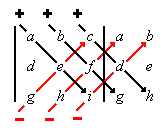
\includegraphics[scale=0.6]{sarrus}\\

\textbf{arithmetic rules:}\\
$\det (A \cdot B) = \det (A) \cdot \det (B)$\\
$\det (A^{-1}) = \frac 1 {\det (A)}$\\
$\det\left(rA\right) = r^n\det A\,\,$,  for all $A^{n\times n}$ and scalars $r$

\subsection{eigenvalues, eigenvectors, eigenspace}
1. Calculate \textbf{eigenvalues} by solving $\det\left( A - \lambda I \right) = 0$\\
2. Any vector $x$ that satisfies $\left(A - \lambda_i I\right) x = 0$ is \textbf{eigenvector} for $\lambda_i$.
3. $\text{Eig}_A(\lambda_i) = \{x \in\mathbb{C}^n\,:\, (A -  \lambda_i) x = 0\}$ is \textbf{eigenspace} for $\lambda_i$.

\subsection{definiteness}

\subsection{obvious properties}
\textbf{square}: $N \times N$\\
\textbf{symmetric}: $A = A^T$\\
\textbf{diagonal}: 0 except $a_{kk}$\\
$\Rightarrow$ implies triangular (eigenvalues on main diagonale)
\subsection{orthogonal}
$A^T = A^{-1}$

\subsection{nonsingular}
A is nonsingular = invertible = regular iff:\\
\begin{list}{}
\item There is a matrix $B := A^{-1}$ such that $AB = I = BA$.
\item $det(A) \ne 0$
\item T$Ax = b$ has exactly one solution for each b.
\item The columns of $A$ are linearly independent.
\end{list}
\smallbreak
$\Rightarrow det(A)^{-1} = det(A^{-1})$\\
$\Rightarrow (A^{-1})^{-1} = A$\\
$\Rightarrow (A^{T})^{-1} = (A^{-1})^{T}$

\subsection{diagonalizable}
$A^{N \times N}$ can be diagonalized iff it has $n$ linear independant eigenvectors.
Then, there is an invertible $T$, such that:
\[
D := T^{-1}AT=\begin{pmatrix}\lambda_{1}\\
& \ddots\\
& & \lambda_{n}\end{pmatrix}
\]
\[
\begin{array}{ccc}
A = T^{-1}DT & \mathbf{and} & AT=T\begin{pmatrix}\lambda_{1}\\
& \ddots\\
& & \lambda_{n}\end{pmatrix}
\end{array}
\]
T can be created with eigenvectors of A.

\subsection{diagonally dominant matrix}
$\forall i. |a_{ii}| \geq \sum_{j\neq i} |a_{ij}| \quad$
\subsection{Hermitian}
\subsection{triangular}
$\Rightarrow$ Eigenvalues on main diagonale
\subsection{unitary}
$\Rightarrow$ $cond_2(A) = 1$
\subsection{idempotent}
\subsection{adjugate}
\subsection{block matrices}
$\det\begin{pmatrix}A& 0\\ C& D\end{pmatrix} = \det\begin{pmatrix}A& B\\ 0& D\end{pmatrix} = \det(A) \det(D)$

\subsection{rank}
\subsection{kernel}
\subsection{trace}
defined on n$\times$n square matrices: $\mathrm{tr}(A) = a_{11} + a_{22} + \dots + a_{nn}$\\
(sum of the elements on the main diagonal)
\subsection{span}
\subsection{spectrum}
$\sigma(A)=\{\lambda\in\mathbb{C}\,:\,\lambda \text{ is eigenvalue of A}\}$
\end{multicols}
\end{document}